% !TeX root = main.tex

\section{Overview} \label{ovr}

The way I approach any project is to break the system up into small parts then analyze and debug those parts in Matlab. This divide and conquer gives me a greater understanding of the parts and increases the chances of code working immediately once incorporated into the glsl. I will make the code available as I progress so that those involved can progress along with me. This will also provide a learning path for anyone joining the project at a later date. I don't want to become indispensable. The approach at every stage is tentative and I will await review before continuing.

\section{Rigid Fiber P001} \label{p001}

The first step in this project is to determine the structure of a rod. 
\Figo{RodStructure} shows a single rod containing 5 particles. 
\begin{figure}[H]
\centering
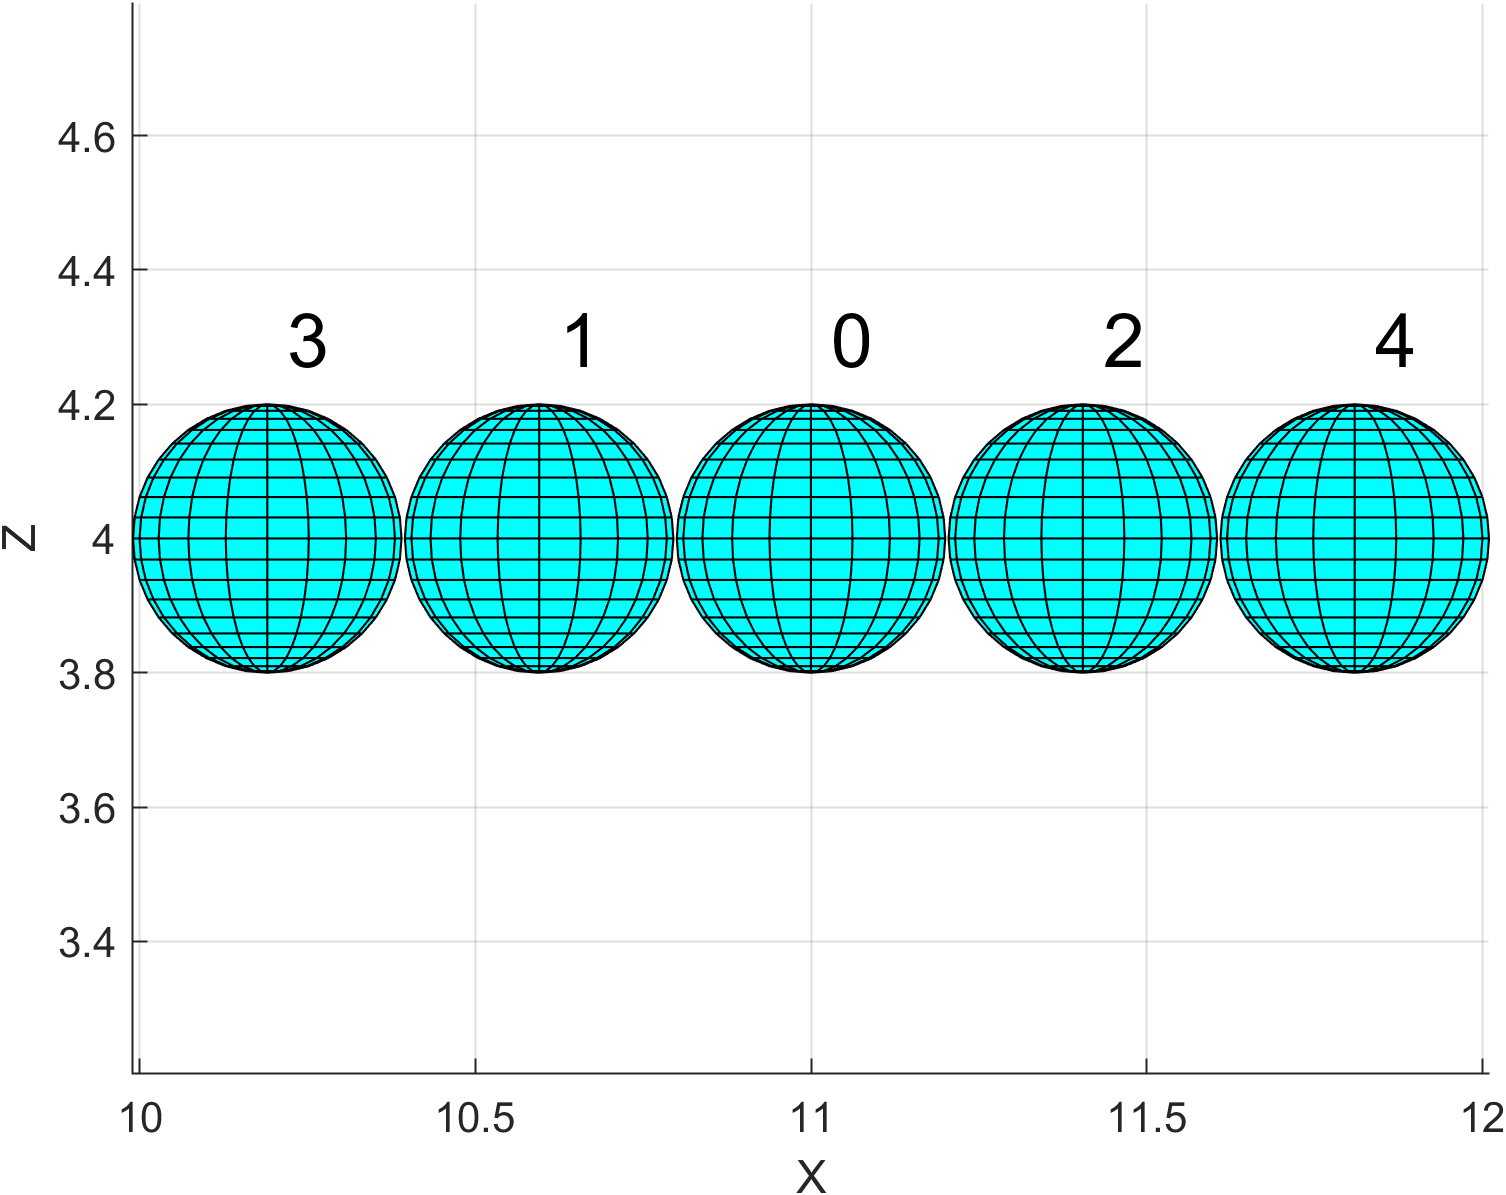
\includegraphics[width=3.40in]{../../../../RCCDRigidFiber/images//RodStructure1.png}
\captionof{figure}[Single Ros.]{\textit{A single rod showing the structure}}
\label{fig:RodStructure}
\end{figure}


Each rod has a \textit{rod number}, \texttt{rnum}, an \textit{in rod} particle, or \textit{member}, number \texttt{inum}, and the number of particles that constitute the rod, \texttt{N}. Each particle continues to have a unique particle ID, \texttt{pnum}.
 
The tentative rules are:
\begin{itemize}
\item The rod particles do not overlap since they are part of the same structure and this would waste collision detection for parts we know are already bonded.
\item The central particle has its origin at the center of mass and \texttt{inum} is equal to 0.
\item The particles to the left of the central particle have even numbered \texttt{inum}.
\item The particles to the right of the central particle have odd numbered \texttt{inum}.
\item This means that the number of particles that make up a rod, \texttt{N}, are always odd.
\item The particles will not overlap and we can use a three dimensional momentum equation to 'impulse' the particles back to their boundaries (this can be complicated since one should not use the square root or modulus on a GPU).
\end{itemize}

This will require two compute phases. The first compute will be threaded by particle and calculates individual particle collisions and reactions (by processing the \textit{potentially colliding set},(PCS) constructed by the graphics phase. The next compute phase will will be threaded by rod number and will calculate the reaction of the whole rod due to collision reactions of its member particles. The efficienty here is that once the collisions are processed in the first compute run, the collisions are stored in memory and we do not need to do it again. 

The change in position of the rod is calculated in the vertex phase. This is due to the fact that we cannot change the position of particle in the compute phase as this would corrupt the collision queries.



